\documentclass[11pt]{article}

% ---------- Packages ----------
\usepackage[margin=1in]{geometry}
\usepackage{amsmath, amssymb}
\usepackage{graphicx}
\usepackage{fancyhdr}
\usepackage{float}
\usepackage{listings}
\usepackage{xcolor}
\usepackage{cancel}
\usepackage[normalem]{ulem}

% ---------- MATLAB Code Listing Style ----------
\lstdefinestyle{matlab}{
    language=Matlab,
    basicstyle=\ttfamily\footnotesize,
    breaklines=true,
    breakatwhitespace=false,
    postbreak=\mbox{$\hookrightarrow$\space},
    columns=fullflexible,
    keepspaces=true,
    frame=none,
    numbers=left,
    numberstyle=\tiny,
    showstringspaces=false
}
\lstset{style=matlab}

% ---------- Paragraph Formatting ----------
\setlength{\parindent}{0pt}
\setlength{\parskip}{0.5em}

% ---------- Header ----------
\pagestyle{fancy}
\fancyhf{}
\lhead{ASEN 5335 Aerospace Environment}
\rhead{Justin Le}
\cfoot{\thepage}

% ---------- Document ----------
\begin{document}

% ---------- Title ----------
\begin{center}
    {\Large \textbf{Homework 2}}\\[0.5em]
    {\large ASEN 5335 Aerospace Environment}\\[0.5em]
    Justin Le\\
    \today
    \\[0.5em]
\end{center}

\vspace{1em}

\section*{Problem 1: Spaceballs}
\subsection*{(i.)}
\hspace*{2em}We are able to use the provided MSISatmosphere1000.m profile to calculate the
an approximate total mass of the atmosphere. The MSISatmosphere1000 function
takes inputs of altitudes and outputs a structure, one of which is mass density which
corresponds to that altitude. Using MATLAB we are able to have a vector of altitudes that
range to 1000 km, the maximum model input of the MSISatmosphere1000 function. We can then
obtain a vector of mass densities $\rho$. We use the following,
\[
\begin{gathered}
m = \rho V \\
m = \int{\rho dV} \\
\text{And for a sphere,} \\
m = \int{\rho*4\pi r^2 dr} \\
\therefore m = 4\pi\int{\rho r^2dr}
\end{gathered}
\]
\hspace*{2em}With $\rho$ being a vector and $r$ also being a vector of radius of this atmospheric
shell (altitude including radius of the Earth $R_E = 6371 \, \mathrm{km}$), we can integrate
within MATLAB to obtain a $\boxed{m=5.297*10^{18}\,\mathrm{kg}}$.
\subsection*{(ii.)}
\hspace*{2em}Assuming a volume of $V = 10*10^3*10*10^3*100*10^3 = 1*10^{13} \, \mathrm{m^3}$, a constant temperature $T = 300 \, \mathrm{K}$, molar mass $M = 0.029 \, \mathrm{kg/mol}$,
and universal gas constant $R = 8.314 \, \mathrm{J/(molK)}$. We can use the ideal gas law,
\[
\begin{gathered}
PV = \frac{m}{M}\\
\text{Rewrite to solve for pressure $P$,} \\
P = \frac{m}{MV}RT \\
\boxed{P = 4.556*10^{10} \, \mathrm{Pa}}
\end{gathered}
\]

\newpage
\section*{Problem 2: Atmospheric Scale Height}
\hspace*{2em}To calculate the scale height $H$ of air mixture assuming $N_2/O_2$ mixture
at sea level, we use the equation.
\[
\begin{gathered}
H = \frac{kT}{mg}
\end{gathered}
\]
\hspace*{2em}Where we assume a constant $T = 300 \, \mathrm{K}$ from the problem, and $k = 1.38*10^{-23} \, \mathrm{J/K}$,
the Boltzmann constant, $g = 9.81 \, \mathrm{m/s^2}$, the gravitational constant. We then
seek the molecular mass of $N_2/O_2$ mixture. This can be obtained from the table provided
in the HW. We find the atomic mass of the air mixture provided with the \% by volume
\[
\begin{gathered}
\cancel{amu_{air} = 28.0134\left(.781\right)+31.9988\left(.209\right) = 28.566\, \mathrm{g/mol}} \\
\cancel{m_{air} = amu_{air}*\frac{1 \, \mathrm{kg}}{1000\, \mathrm{g} * 6.02*10^{23}\, \mathrm{g/mol}}} \\
\cancel{m_{air} = 4.745*10^{-26} \, \mathrm{kg}} \\
\textcolor{red}{\text{We also include Argon (} \approx 0.93\%\text{).}} \\
\textcolor{red}{amu_{air} \approx 28.96 \, \mathrm{g/mol}} \\
\textcolor{red}{m_{air} = amu_{air}*\frac{1 \, \mathrm{kg}}{1000\, \mathrm{g} * 6.02*10^{23}\, \mathrm{g/mol}} \approx 4.811*10^{-26} \, \mathrm{kg}}
\end{gathered}
\]

\hspace*{2em}This process of finding molecular weight and converting it can be repeated for
atomic Oxygen, helium, and hydrogen.
\[
\begin{gathered}
amu_{oxygen} = (31.9988 \, \mathrm{g/mol}) / 2 = 15.9994 \, \mathrm{g/mol} \\
amu_{helium} = 4.0026  \, \mathrm{g/mol} \\
\cancel{amu_{hydrogen} = 2.01594  \, \mathrm{g/mol}}
\\
\textcolor{red}{\text{For hydrogen use atomic }} \\
\textcolor{red}{amu_{hydrogen} \approx 1.008 \, \mathrm{g/mol} \text{ (atomic H)}}
\\
\\
m_{oxygen} = 2.6577*10^{-26} \, \mathrm{kg} \\
m_{helium} = 6.6488*10^{-27} \, \mathrm{kg} \\
\cancel{m_{hydrogen} = 3.3487*10^{-27} \, \mathrm{kg}} \\
\textcolor{red}{m_{hydrogen} \approx 1.674*10^{-27} \, \mathrm{kg}}
\end{gathered}
\]

\hspace*{2em}The scale height equation can be used with each respective molecular mass of
the species in question.
\[
\begin{gathered}
\boxed{\cancel{H_{air} = 8.8938*10^3 \, \mathrm{m}}} \\
\textcolor{red}{\text{including Argon}} \\
\boxed{H_{air} \approx 8.79*10^{3} \, \mathrm{m}} \\
\boxed{H_{oxygen} = 1.588*10^4 \, \mathrm{m}} \\
\boxed{H_{helium} = 6.347*10^4 \, \mathrm{m}} \\
\boxed{\cancel{H_{hydrogen} = 1.2602*10^5 \, \mathrm{m}}} \\
\textcolor{red}{\text{using atomic H}} \\
\boxed{H_{hydrogen} \approx 2.52*10^{5} \, \mathrm{m}}
\end{gathered}
\]


\begin{figure}[H]
    \centering
    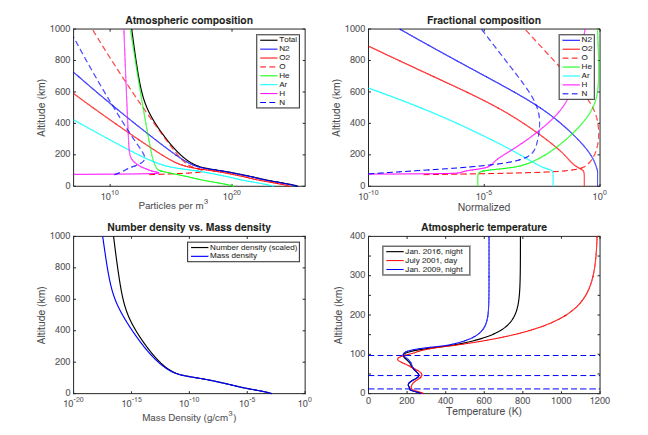
\includegraphics[width=0.8\textwidth]{atmospheric_profile.png}
    \caption{Atmospheric Profile}
    \label{fig:atmospheric_profile}
\end{figure}

\begin{figure}[H]
    \centering
    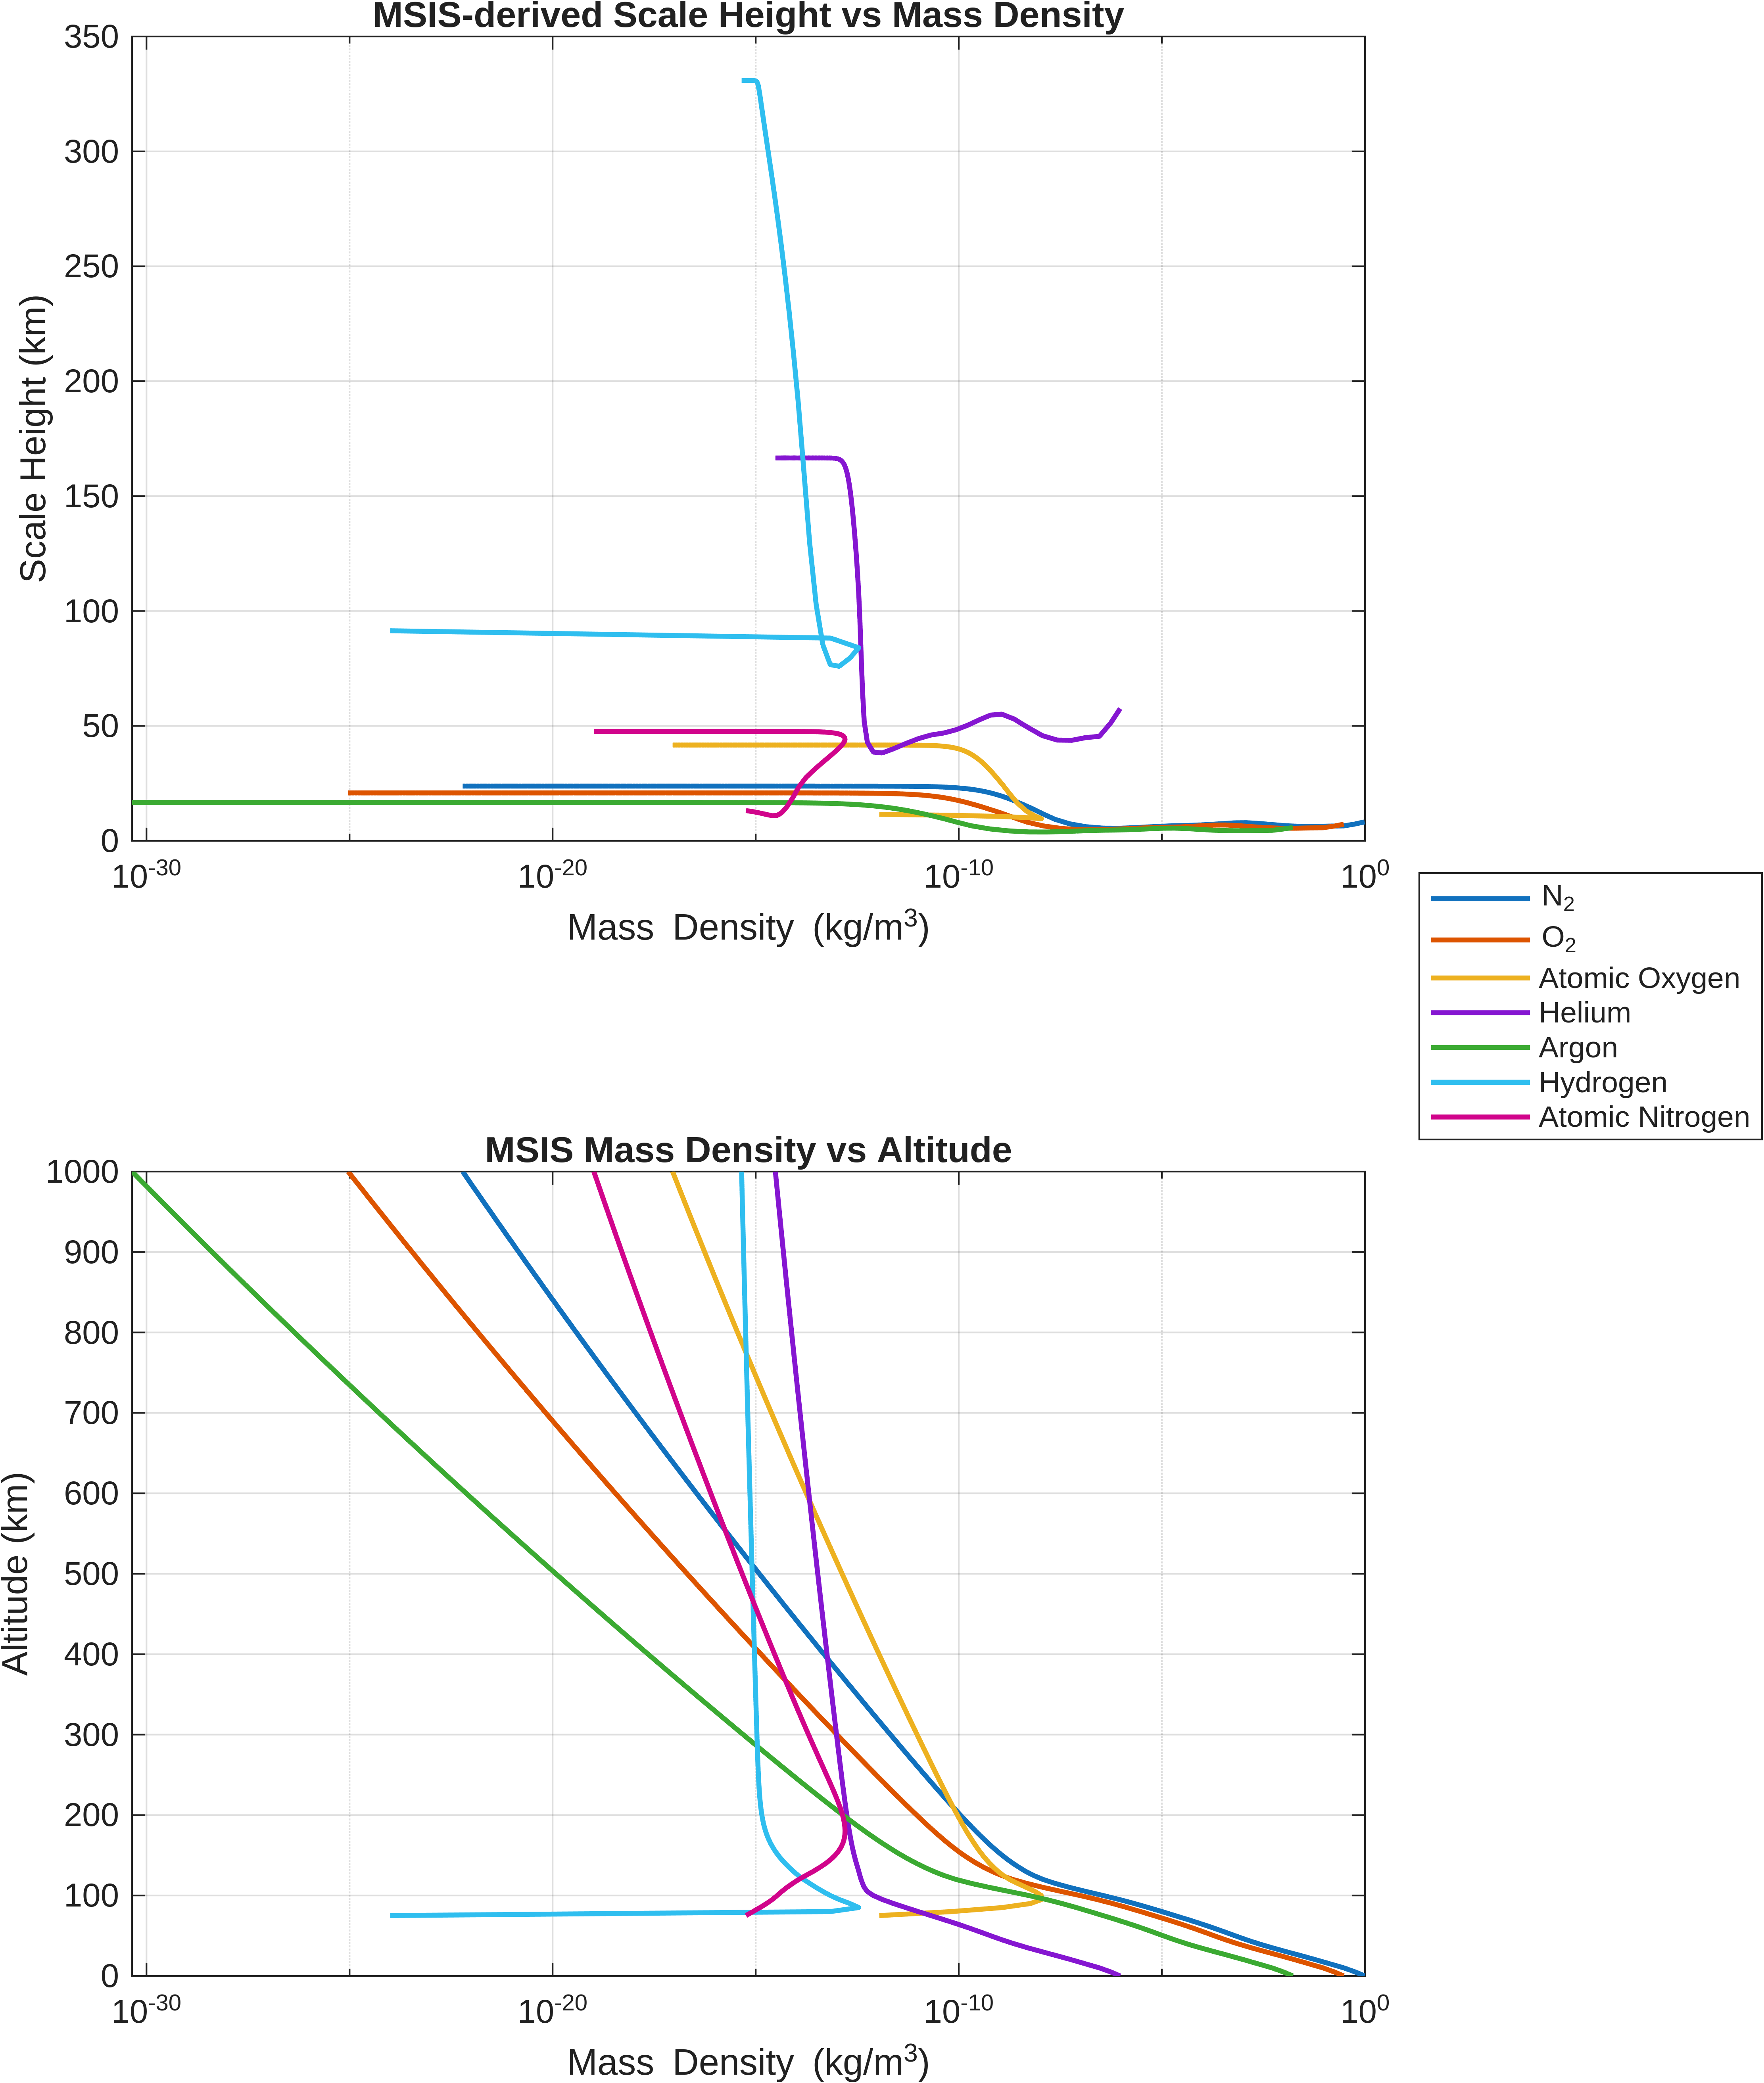
\includegraphics[width=0.8\textwidth]{HW2Problem2_scaleheight_vs_altitude.png}
    \caption{Density vs Scale Height and Altitude of Atmospheric Species}
    \label{fig:scaleheight_vs_altitude}
\end{figure}
\hspace*{2em}We seek to also calculate scale height from the MSIS profiles. From the MSIS
profiles there will be different temperatures instead of the fixed $T$ used earlier. This
can be done in MATLAB, which is shown in Figure \ref{fig:scaleheight_vs_altitude}. From here, we can
observe that MSIS profile for altitude matches up with the figure provided in the assignment. We can
also observe the relation between scale height and the altitudes of each species. Scale height increases
as density and altitude increase.

\textcolor{red}{We can also compare quantitatively by taking the derivative of log of density vs. altitude on
the MSIS plot. This gives local scale height at every altitude. The mismatch is mostly from assuming constant $T=300\,\mathrm{K}$
, which raises the actual scale height in the atmosphere.}

\newpage
\section*{Problem 3: Atmosphere Variation}
\subsection*{(i.)}
\begin{figure}[H]
    \centering
    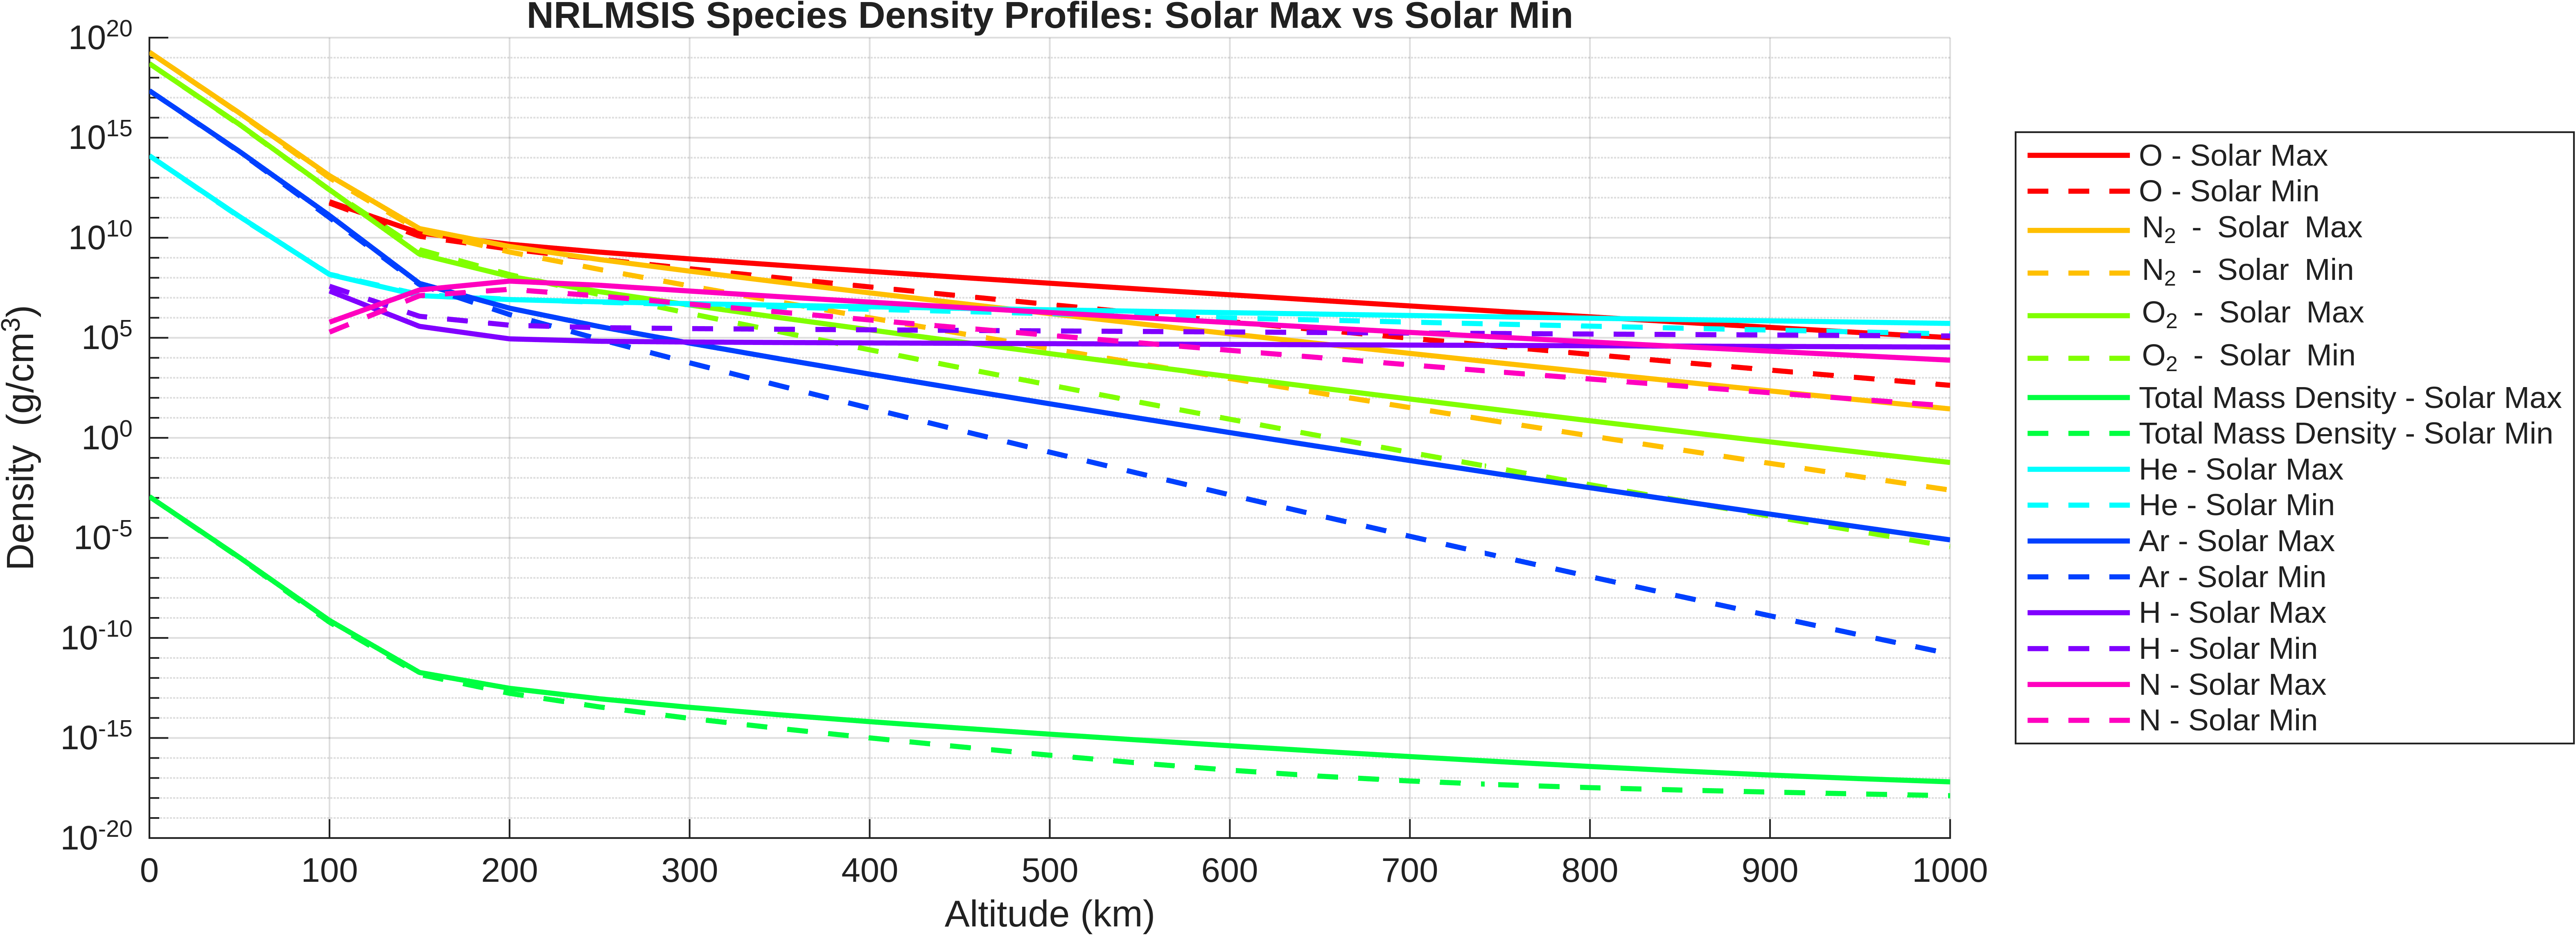
\includegraphics[width=0.8\textwidth]{NRLMSIS_Species_Density_Profiles.png}
    \caption{NRLMSIS Species Density Profiles Solar Max vs Solar Min}
    \label{fig:NRLMSIS_Species_Density_Profiles}
\end{figure}

\subsection*{(ii.)}
\hspace*{2em}At 600 km, there is variation between the solar maximum and solar minimum with the
density profiles of each species deviating. At solar maximums, the densities of each
species tends to be larger by multiple orders of magnitude than they would be a solar minimums.
This can even be soon overall with the Total Mass Density variation between solar maximums and
minimums. The implication of this for spacecraft operations is that there will be different atmospheric conditions
for spacecraft depending on if it is a solar maximum or minimum. For instance, drag will be
dependent on the density of the atmosphere, during solar maximums where density can increase
by multiple orders of magnitude, drag will also be considerably affected. This could especially
impact LEO orbits with their orbits being considerably influenced by drag. Their satellite operations
could therefore vary depending on if it is a solar maximum or minimum.

\subsection*{(iii.)}
\hspace*{2em}The dominant atmospheric species would be O, atomic oxygen, \sout{for both solar
maximum and solar minimum.}

\textcolor{red}{This is the case for solar maximum. At solar minimum, we instead find Helium (He)
to be the dominant species.}

\newpage
\section*{Problem 4: Oxygen Impact}
\subsection*{(i.)}
\hspace*{2em}To find the characteristic velocity of an oxygen atom O at $T = 1000 \, \mathrm{K}$ in the thermosphere,
we are able to use the Maxwell Boltzmann Characteristic RMS Velocity equation.
\[
\begin{gathered}
v_{rms} = \sqrt{ \frac{3k_B T}{m} }
\end{gathered}
\]
\hspace*{2em}$k_B = 1.38*10^{-23} \, mathrm{m^2 kg / s^2 K}$ as the Boltzmann constant, and
we are able to find $m = 2.657*10^{-26} \, \mathrm{kg}$ for an oxygen atom. We can plug this
into the equation to simply find,
\[
\begin{gathered}
\boxed{v = 1248.26 \, \mathrm{m/s}}
\end{gathered}
\]

\subsection*{(ii.)}
\hspace*{2em}We then calculate the velocity that a
spacecraft in LEO at 600 km would have,
\[
\begin{gathered}
v_{orbit} = \sqrt{\frac{GM_{Earth}}{r}} \\
G = 6.67*10^{-11} \, \mathrm{Nm^2/kg^2} \\
M_{Earth} = 5.972*10^{24} \, \mathrm{kg} \\
r = 600*10^3 \, \mathrm{m} + 6371*10^3 \, \mathrm{m} = 6671*10^3 \, \mathrm{m} \\
\therefore v_{orbit} = 7559 \, \mathrm{m/s}
\end{gathered}
\]

The energy imparted onto the spacecraft by an oxygen atom would be using the mass
of the oxygen atom and the velocity of the spacecraft,
\[
\begin{gathered}
KE = \frac{1}{2} m_{oxygen} v_{orbit}^2 \\
KE = 7.591*10^{-19} J \\
\text{Where $1\, \mathrm{J}$ = $6.242*10^{18} \, \mathrm{eV}$} \\
\boxed{\therefore KE = 4.738 \, \mathrm{eV}}
\end{gathered}
\]

\subsection*{(iii.)}
\hspace*{2em}Examine the energy threshold for $Al$ being bombarded by $O$ from
the table, we find $E_th = 23\,\mathrm{eV} = 3.685*10^{-18}\,\mathrm{J}$. Rewrite
the kinetic energy equation to find velocity required for this energy threshold,
\[
\begin{gathered}
v_{th} = \sqrt{\frac{2 E_{th}}{m_O}} \\
v_{th} = 16654.76 \, \mathrm{m/s} = 16.654\,\mathrm{km/s}
\end{gathered}
\]

\hspace*{2em}We now want to find the fraction of the Maxwell Boltzmann distribution
for atomic oxygen that would have velocities higher than this. \sout{We use the diagram provided in
the slides to approximate that it would be ~$0.01\%$ of the atomic oxygen would have sufficient energy
to cause sputtering.}

\textcolor{red}{By subtracting the spacecraft's own orbital velocity from the velocity threshold calculated earlier,
$v_{th} - v_{orbit} \approx 16.654 - 7.559 \approx 9 \, \mathrm{km/s}$. We could then integrate the
Maxwell-Boltzmann distribution above that with a factor of $\frac{1}{2}$ assuming only one side is impacted,
this will give a fraction of about
$2.23\times10^{-34}$, therefore there is minimal sputtering impact on the spacecraft.}

\newpage
\section*{Problem 5: Orbit Decay}
\subsection*{(i.)}
\[
\begin{gathered}
\text{We use the following relations:} \\
F_{drag} = \frac{1}{2} \rho V^2 C_D A, \qquad
V = \sqrt{\frac{G M_E}{a}}, \qquad
P^2 G M_E = 4 \pi^2 a^3
\end{gathered}
\]

\[
\begin{gathered}
\textbf{Step 1:} \text{ Drag equation} \\
m \frac{dV}{dt} = \frac{1}{2} \rho V^2 C_D A \\
\frac{dV}{dt} = \frac{\rho V^2 C_D A}{2m}
\end{gathered}
\]

\[
\begin{gathered}
\textbf{Step 2:} \text{ Relate } da/dt \text{ to } dV/dt \text{ with the velocity equation} \\
V^2 a = G M_E \\
\left(\frac{d}{dt}\right)\Big(V^2 a\Big) = \left(\frac{d}{dt}\right)\Big(G M_E\Big) \\
2Va\,\frac{dV}{dt} + V^2 \frac{da}{dt} = 0 \\
\frac{da}{dt} = -\frac{2a}{V}\frac{dV}{dt} \\
\text{Substituting Step 1,} \\
\frac{da}{dt} = -\frac{2a}{V}\left(\frac{\rho V^2 C_D A}{2m}\right) \\
\frac{da}{dt} = -\frac{a \rho V C_D A}{m}
\end{gathered}
\]

\[
\begin{gathered}
\textbf{Step 3:} \text{ Relate } da/dt \text{ to } dP/dt \text{ with Kepler's third law} \\
P^2 G M_E = 4 \pi^2 a^3 \\
\left(\frac{d}{dt}\right)\Big(P^2 G M_E\Big) = \left(\frac{d}{dt}\right)\Big(4 \pi^2 a^3\Big) \\
2P\,G M_E\,\frac{dP}{dt} = 12\pi^2 a^2 \frac{da}{dt} \\
\frac{da}{dt} = \frac{P\,G M_E}{6 \pi^2 a^2}\,\frac{dP}{dt}
\end{gathered}
\]

\[
\begin{gathered}
\textbf{Step 4:} \text{ Setting the two expressions for $da/dt$ equal,} \\
-\frac{a \rho V C_D A}{m} = \frac{P\,G M_E}{6 \pi^2 a^2}\,\frac{dP}{dt} \\
\frac{dP}{dt} = -\frac{6 \pi^2 a^3 \rho V C_D A}{m\,P\,G M_E} \\
\text{Using } GM_E = V^2 a \text{ to eliminate } GM_E, \\
\frac{dP}{dt} = -\frac{6 \pi^2 a^3 \rho V C_D A}{m\,P\,V^2 a} \\
\frac{dP}{dt} = -\frac{6 \pi^2 a^2 \rho C_D A}{m\,P\,V} \\
\text{For a circular orbit, } 2\pi a = PV, \\
\frac{dP}{dt} = -\frac{6 \pi^2 a^2}{m\,(2\pi a)}\,\rho C_D A \\
\frac{dP}{dt} = -\frac{3 \pi a \rho C_D A}{m}
\end{gathered}
\]
\[
\boxed{\frac{dP}{dt} = -3 \pi a \rho \frac{C_D A}{m}}
\]
\subsection*{(ii.)}
\hspace*{2em} See section at end of assignment for full MATLAB Code.
\begin{figure}[H]
    \centering
    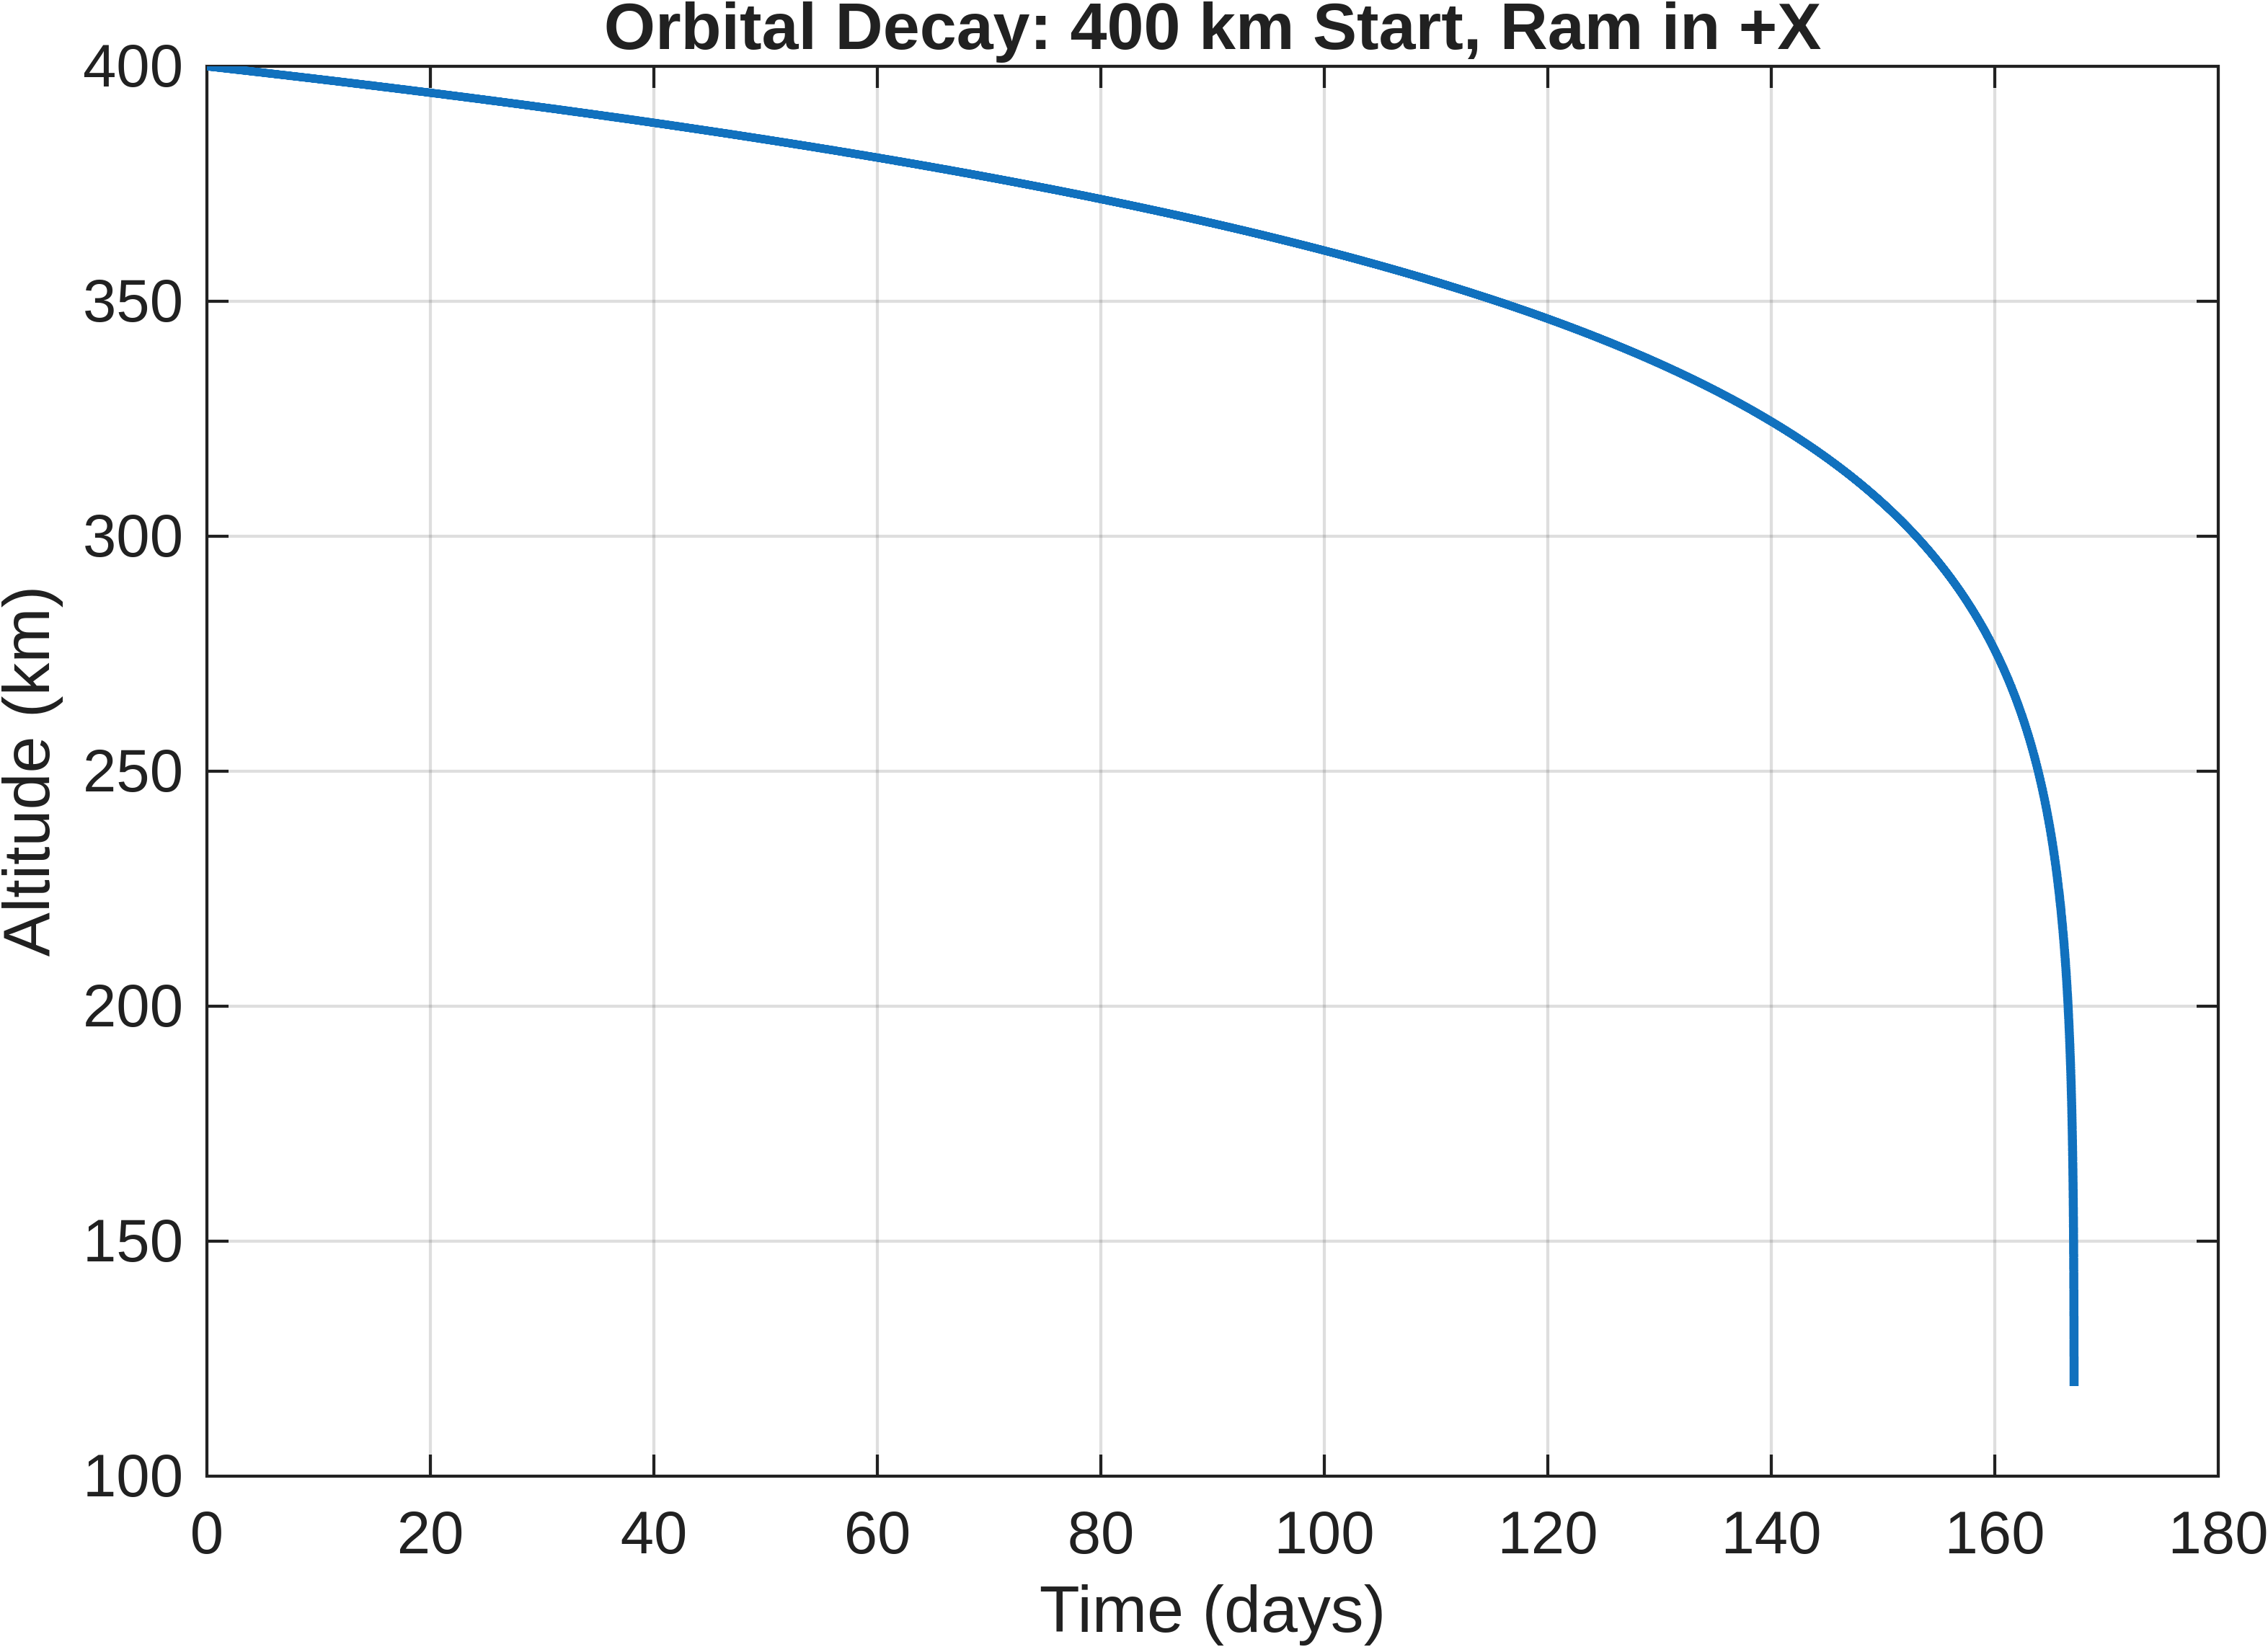
\includegraphics[width=0.6\textwidth]{HW2Problem5_OrbitDecay_400km_x.png}
    \caption{Orbital Decay for 400 km in +x}
    \label{fig:HW2Problem5_OrbitDecay_400km_x}
\end{figure}

\textcolor{red}{\boxed{\text{Deorbit time} \approx 167 \text{ days}}}

\subsection*{(iii.)}
\begin{figure}[H]
    \centering
    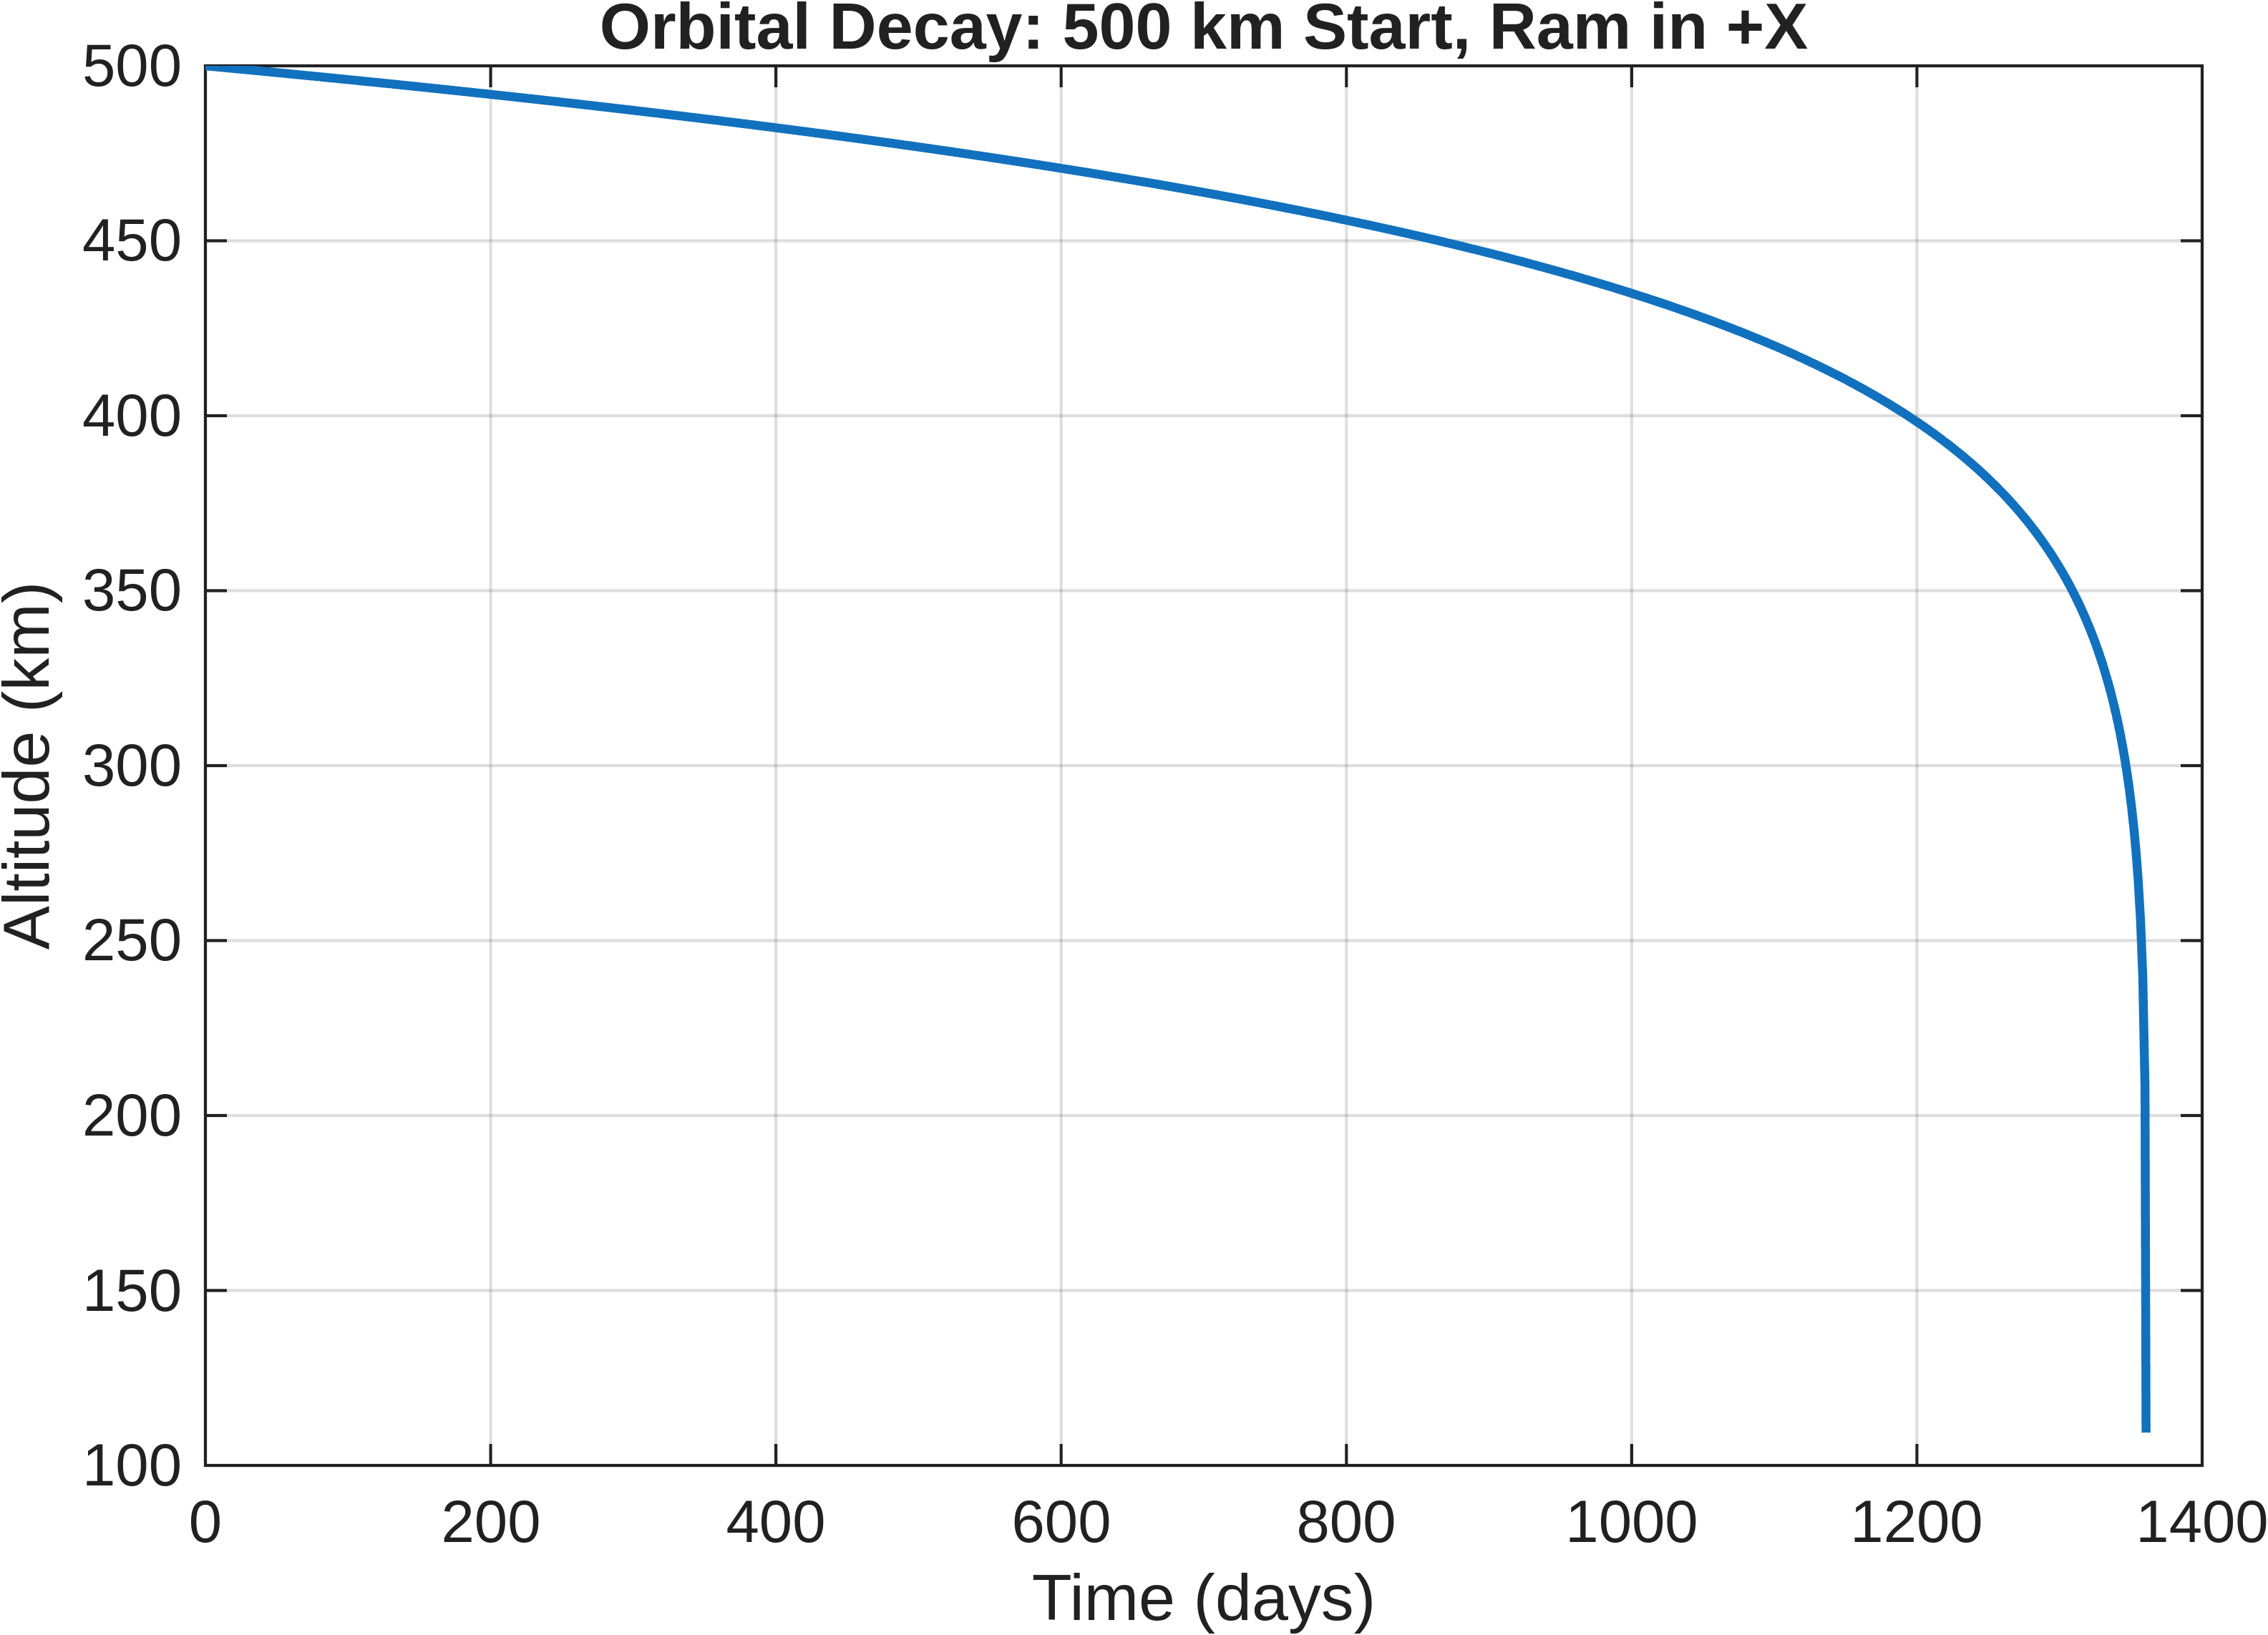
\includegraphics[width=0.6\textwidth]{HW2Problem5_OrbitDecay_500km_x.png}
    \caption{Orbital Decay for 500 km in +x}
    \label{fig:HW2Problem5_OrbitDecay_500km_x}
\end{figure}

\textcolor{red}{\boxed{\text{Deorbit time} \approx 1360 \text{ days}}}

\subsection*{(iv.)}
\begin{figure}[H]
    \centering
    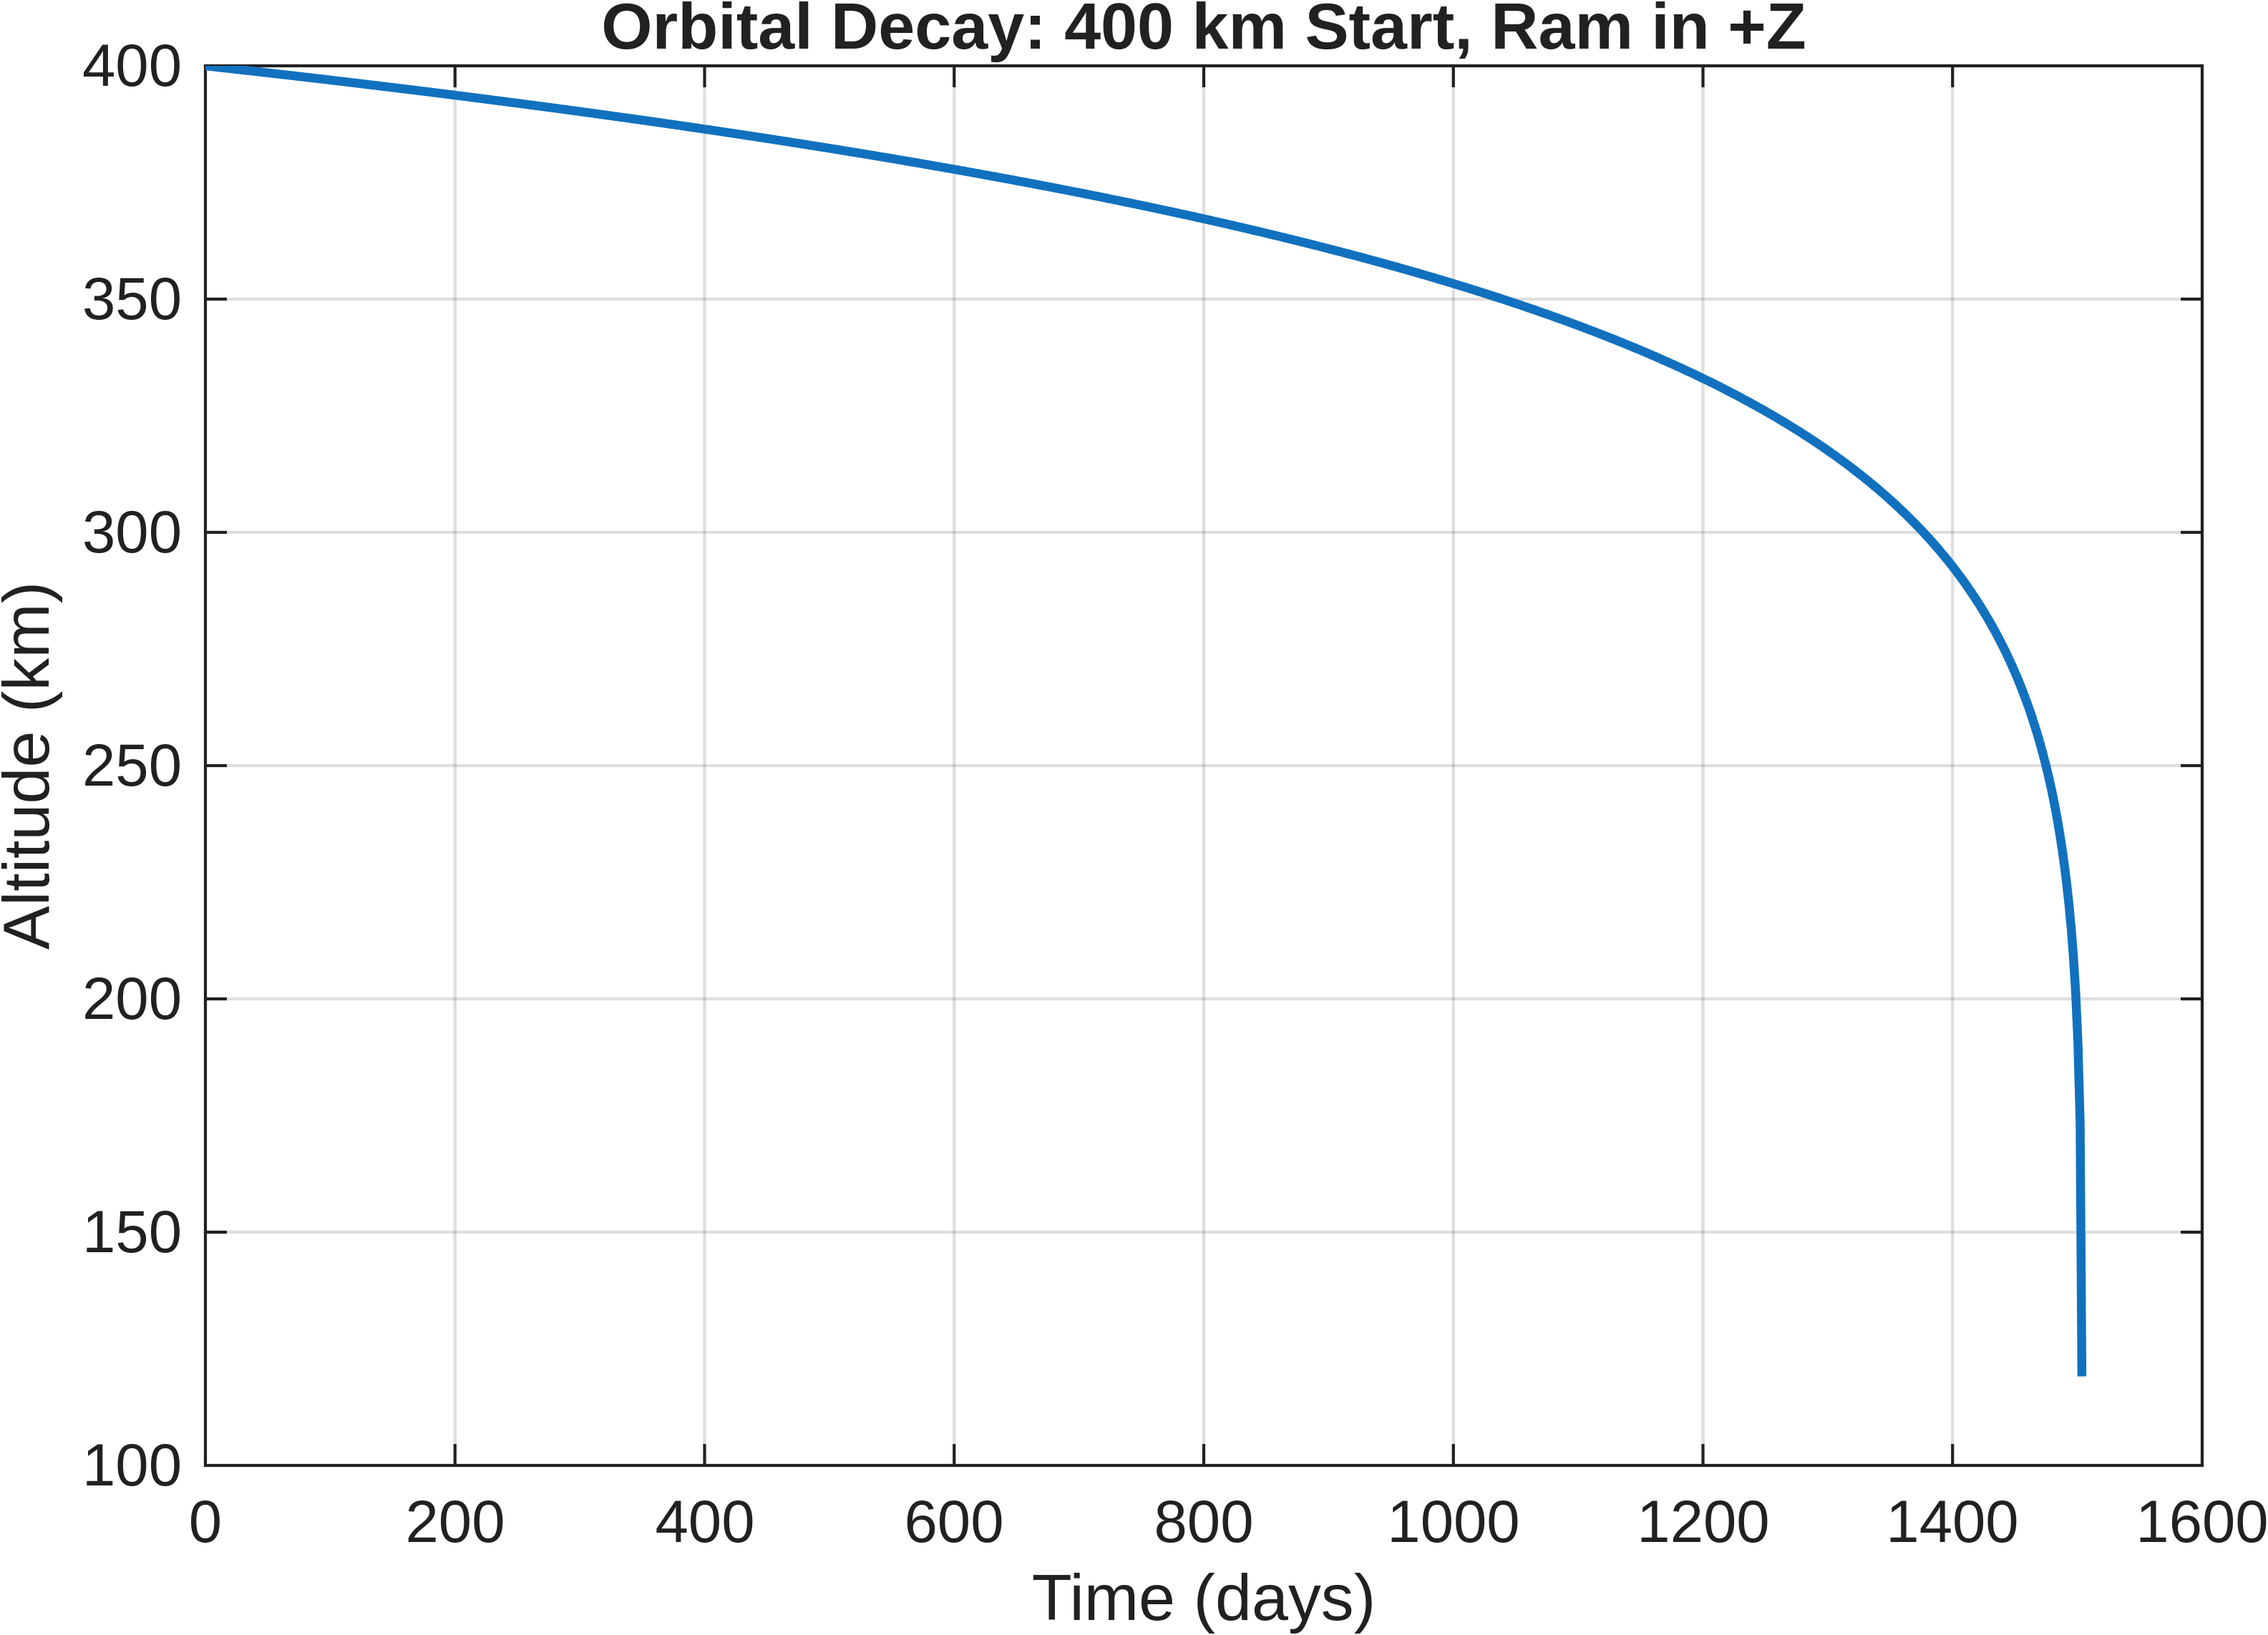
\includegraphics[width=0.6\textwidth]{HW2Problem5_OrbitDecay_400km_z.png}
    \caption{Orbital Decay for 400 km in +z}
    \label{fig:HW2Problem5_OrbitDecay_400km_z}
\end{figure}

\textcolor{red}{\boxed{\text{Deorbit time} \approx 1502 \text{ days}}}

\newpage
\section*{Problem 6: Atmosphere Uncertainty and Neutral Winds}
\subsection*{(i.)}
\begin{figure}[H]
    \centering
    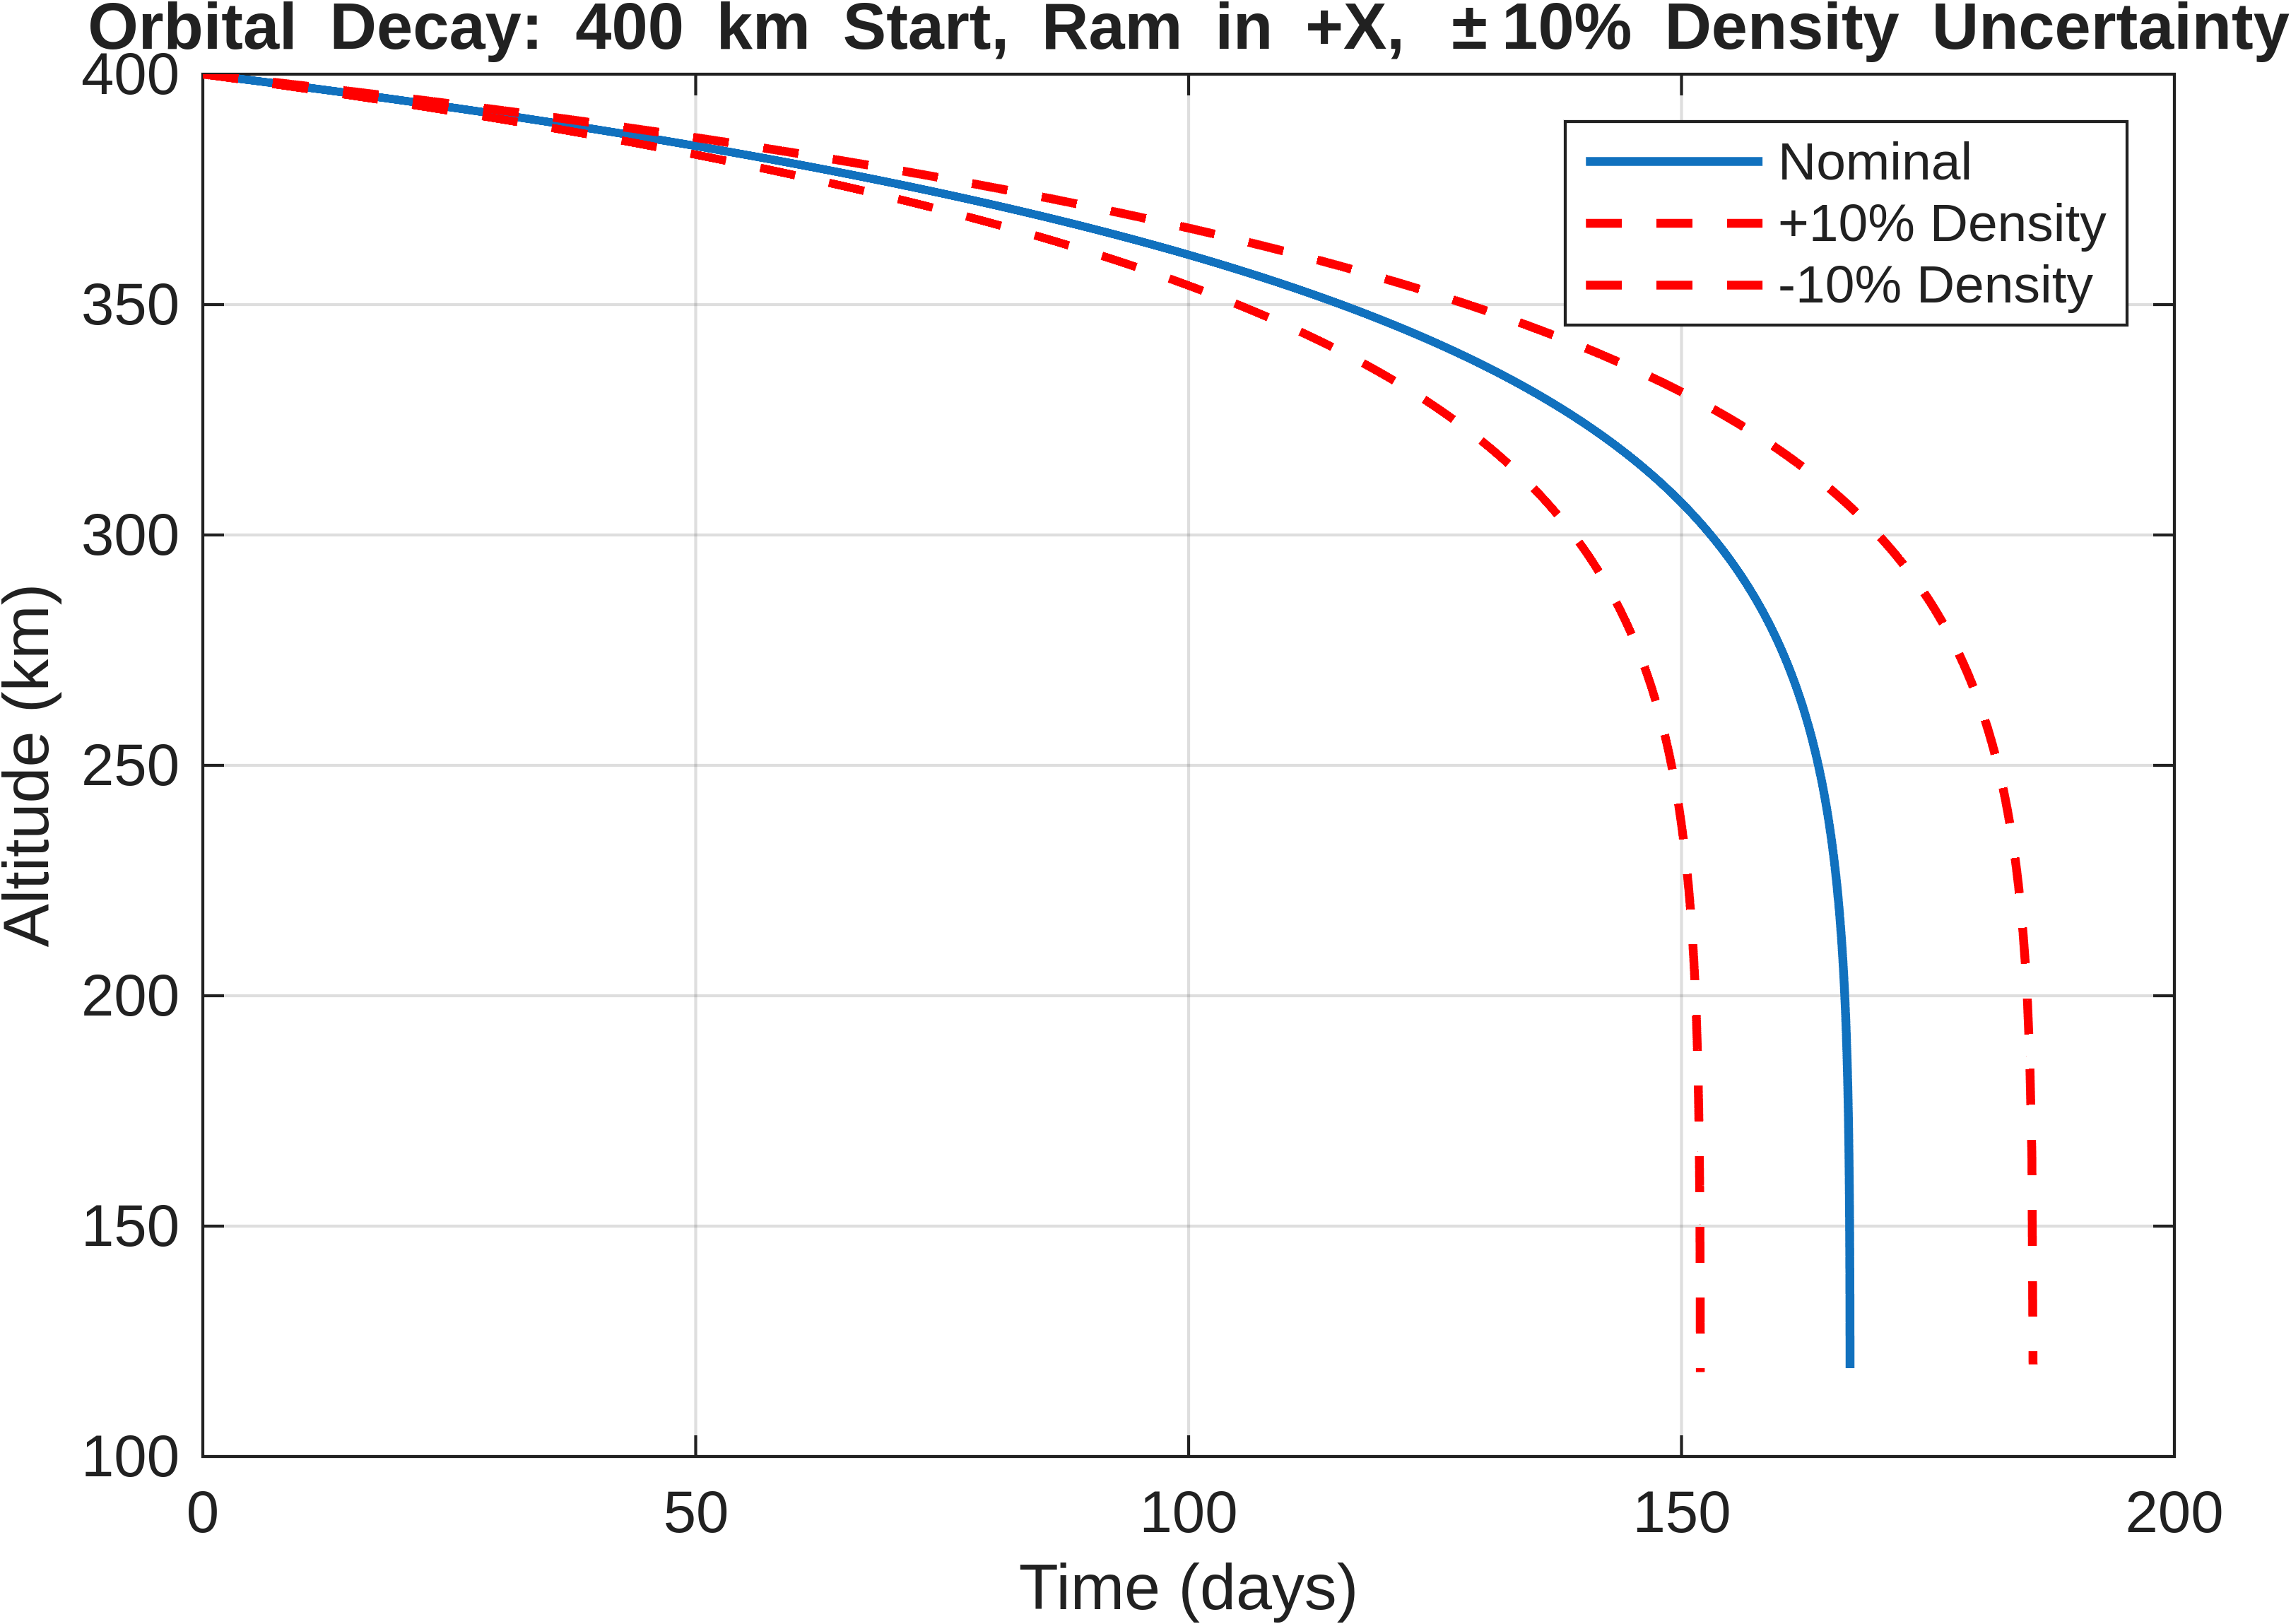
\includegraphics[width=0.6\textwidth]{HW2Problem6_OrbitDecay_400km_x_uncertainty.png}
    \caption{Orbital Decay for 400 km in +z with 10\% Uncertainty}
    \label{fig:HW2Problem5_OrbitDecay_400km_uncertain_z}
\end{figure}

\hspace*{2em}We are able to observe a difference in deorbit time of between
33 and 34 days based on the upper and lower bounds of density uncertainty.
\subsection*{(ii.)}
\hspace*{2em}Given a 90 minute orbit around Earth at some LEO altitude where this
cubesat is operating, the implications for where this spacecraft re entry point in the
atmosphere is that there is massive uncertainty in where it will re enter the atmosphere
over it's entire ballistic deorbiting process. This location would greatly vary due to
this uncertainty.

\newpage
\section*{Problem 7: Air Breathing Thruster}
\subsection*{(i.)}
\hspace*{2em}In order to find the thrust required fo balance
the drag force for some spacecraft operating at 400 km, with $C_D = 2.2$
and $A=100\,\mathrm{cm^2}=0.01\,\mathrm{m^2}$, we would start with the drag equation,
\[
\begin{gathered}
F_D = \frac{1}{2}\rho V^2 C_D A \\
\text{This means we seek to also solve for velocity and $\rho$} \\
\text{Solve velocity with the circular orbit relation from Kepler's Law} \\
v = \sqrt{\frac{GM_E}{r}} \text{, where } r = (400*10^3\,\mathrm{m} + 6371*10^3\,\mathrm{m}) \\
v = 7700\,\mathrm{m/s} \\
\text{We can obtain the density at 400 km using the MATLAB function MSISatmosphere1000,} \\
\rho = 1.194*10^{-15}\,\mathrm{g/cm^3} = 1.194*10^{-12}\,\mathrm{kg/m^3} \\
\therefore F_D = 7.787*10^{-7}\,\mathrm{N} = 0.7787\,\mathrm{\mu N}\\
\boxed{\therefore F_T = F_D = 0.7787\,\mathrm{\mu N}}
\end{gathered}
\]

\subsection*{(ii)}
\hspace*{2em} Now to find the exhaust velocity, we can use the relation,
\[
\begin{gathered}
F_D = -V_{ex}\frac{dm}{dt} \\
\text{since } \frac{dm}{dt} \text{ must be equal to the mass collection rate, it is }
\frac{dm}{dt} = \rho VA \text{, at the inlet} \\
\therefore \frac{dm}{dt} = 9.194*10^{-11}\,\mathrm{m/s} \\
V_{ex} = -F_D/\frac{dm}{dt} \\
\boxed{V_{ex} = -8570\,\mathrm{m/s}}
\end{gathered}
\]

\newpage
\section*{Problem 8: Missions}
\hspace*{2em} The method I chose was using space based accelerometer measurements to measure drag and determine atmospheric density.
A mission that implemented this was CHAMPS, basically how the method works is that from $F_D = \tfrac12\rho V^2 C_D A$,
the drag equation, if you were to understand the vehicle's $C_D$, $A$, and $V$, you can measure the deceleration that the
spacecraft is experiencing with accelerometers on board and therefore back out density at some given instance of time. Examining
CHAMPS, it was a german spacecraft that was designed to measure Earth's gravity field, magnetic field, and the ionosphere. CHAMPS'
accelerometer was located at the center of mass of the spacecraft, and it would be measuring all the non-gravitational accelerations with high resolution.
By filtering out the gravitational perturbations, the acceleration that this accelerometer measured would find high resolution mass density of the
atmosphere for CHAMPS' mission duration.

\newpage
\section*{MATLAB Code}

\begin{lstlisting}
%% ASEN 5335 Aerospace Environment
%% Justin Le
%% HW 2 Problem 1

% using MSISatmosphere, function provides mass at some given alt
% integrate over a range to find total mass

alt_km = 0:1:1000; % altitude vector

n = MSISatmosphere1000(alt_km);

rho_kg_m3 = n.mass*1000; % convert g/cm^3 to kg/m^3

R_E_m = 6371e3; % Radius of the Earth
r_m = R_E_m + alt_km*1000; % distance from Earth's center

% Integrate with trapz function, m = 4pi*integral(rho*r^2 dr)
total_atmos_mass = trapz(r_m, 4*pi*rho_kg_m3.*(r_m.^2)) % kg

% Part ii

R = 8.314; % J/molK
T = 300; % K
M = 0.029; % kg/mol
V = 10*10^3*10*10^3*100*10^3; % m^3

P = (total_atmos_mass/(M*V))*R*T % Pa
\end{lstlisting}

\newpage
\begin{lstlisting}
%% ASEN 5335 Aerospace Environment
%% Justin Le
%% HW2 Problem 2

clc;clear; close all

% Constants
k=1.38E-23;
T=300;
g=9.81;

%g/mol to kg conversion
gmol2kg = (1/(1000*6.02E23));

% air
amu_air = 28.0124*(0.781) + 31.9988*(0.209);
m_air = amu_air*gmol2kg;
H_air = (k*T)/(m_air*g)
% atomic oxygen
amu_oxygen = 31.9988/2;
m_oxygen = amu_oxygen*gmol2kg;
H_oxygen = (k*T)/(m_oxygen*g)
% helium
amu_helium = 4.0026;
m_helium = amu_helium*gmol2kg;
H_helium = (k*T)/(m_helium*g)
% hydrogen
amu_hydrogen = 2.01594;
m_hydrogen= amu_hydrogen*gmol2kg;
H_hydrogen = (k*T)/(m_hydrogen*g)

% Convert to km
H_air_km = H_air/1000
H_oxygen_km = H_oxygen/1000
H_helium_km = H_helium/1000
H_hydrogen_km = H_hydrogen/1000

amu_n2 = 28.0134;
amu_o2 = 31.9988;
amu_ar = 39.948;
amu_n = 14.0067;
m_n2 = amu_n2*gmol2kg;
m_o2 = amu_o2*gmol2kg;
m_ar = amu_ar*gmol2kg;
m_n = amu_n*gmol2kg;

% Some range of altitude
alt_range_km = (0:5:1000)';
N = length(alt_range_km);

T_MSIS = zeros(N,1);
n_n2_MSIS = zeros(N,1);
n_o2_MSIS = zeros(N,1);
n_o_MSIS = zeros(N,1);
n_he_MSIS = zeros(N,1);
n_ar_MSIS = zeros(N,1);
n_h_MSIS = zeros(N,1);
n_n_MSIS = zeros(N,1);

% Loop through entire altitude range and return MSIS information
for i = 1:N
    MSIS_i = MSISatmosphere1000(alt_range_km(i));
    T_MSIS(i) = MSIS_i.temp;
    n_n2_MSIS(i) = MSIS_i.n2;
    n_o2_MSIS(i) = MSIS_i.o2;
    n_o_MSIS(i) = MSIS_i.o;
    n_he_MSIS(i) = MSIS_i.he;
    n_ar_MSIS(i) = MSIS_i.ar;
    n_h_MSIS(i) = MSIS_i.h;
    n_n_MSIS(i) = MSIS_i.n;
end

% Density conversions
rho_n2_MSIS = n_n2_MSIS*1e6*m_n2;
rho_o2_MSIS = n_o2_MSIS*1e6*m_o2;
rho_oxygen_MSIS = n_o_MSIS*1e6*m_oxygen;
rho_helium_MSIS = n_he_MSIS*1e6*m_helium;
rho_ar_MSIS = n_ar_MSIS*1e6*m_ar;
rho_hydrogen_MSIS = n_h_MSIS*1e6*m_hydrogen;
rho_n_MSIS = n_n_MSIS*1e6*m_n;

% Calculate scale height
H_n2_MSIS_km = (k*T_MSIS)/(m_n2*g)/1000;
H_o2_MSIS_km = (k*T_MSIS)/(m_o2*g)/1000;
H_oxygen_MSIS_km = (k*T_MSIS)/(m_oxygen*g)/1000;
H_helium_MSIS_km = (k*T_MSIS)/(m_helium*g)/1000;
H_ar_MSIS_km = (k*T_MSIS)/(m_ar*g)/1000;
H_hydrogen_MSIS_km = (k*T_MSIS)/(m_hydrogen*g)/1000;
H_n_MSIS_km = (k*T_MSIS)/(m_n*g)/1000;

% Plotting
figure
tl = tiledlayout(2,1);

nexttile
semilogx(rho_n2_MSIS, H_n2_MSIS_km, 'LineWidth', 1.5, 'DisplayName', 'N_2')
hold on
semilogx(rho_o2_MSIS, H_o2_MSIS_km, 'LineWidth', 1.5, 'DisplayName', 'O_2')
semilogx(rho_oxygen_MSIS, H_oxygen_MSIS_km, 'LineWidth', 1.5, 'DisplayName', 'Atomic Oxygen')
semilogx(rho_helium_MSIS, H_helium_MSIS_km, 'LineWidth', 1.5, 'DisplayName', 'Helium')
semilogx(rho_ar_MSIS, H_ar_MSIS_km, 'LineWidth', 1.5, 'DisplayName', 'Argon')
semilogx(rho_hydrogen_MSIS, H_hydrogen_MSIS_km, 'LineWidth', 1.5, 'DisplayName', 'Hydrogen')
semilogx(rho_n_MSIS, H_n_MSIS_km, 'LineWidth', 1.5, 'DisplayName', 'Atomic Nitrogen')
grid on
xlabel('Mass Density (kg/m^3)')
ylabel('Scale Height (km)')
title('MSIS-derived Scale Height vs Mass Density')

nexttile
semilogx(rho_n2_MSIS, alt_range_km, 'LineWidth', 1.5, 'DisplayName', 'N_2')
hold on
semilogx(rho_o2_MSIS, alt_range_km, 'LineWidth', 1.5, 'DisplayName', 'O_2')
semilogx(rho_oxygen_MSIS, alt_range_km, 'LineWidth', 1.5, 'DisplayName', 'Atomic Oxygen')
semilogx(rho_helium_MSIS, alt_range_km, 'LineWidth', 1.5, 'DisplayName', 'Helium')
semilogx(rho_ar_MSIS, alt_range_km, 'LineWidth', 1.5, 'DisplayName', 'Argon')
semilogx(rho_hydrogen_MSIS, alt_range_km, 'LineWidth', 1.5, 'DisplayName', 'Hydrogen')
semilogx(rho_n_MSIS, alt_range_km, 'LineWidth', 1.5, 'DisplayName', 'Atomic Nitrogen')
grid on
xlabel('Mass Density (kg/m^3)')
ylabel('Altitude (km)')
title('MSIS Mass Density vs Altitude')

lgd = legend('Location', 'eastoutside');
lgd.Layout.Tile = 'east';

set(gcf, 'Units', 'inches', 'Position', [0 0 8 10])
exportgraphics(gcf, 'HW2Problem2_scaleheight_vs_altitude.png', 'Resolution', 600);
\end{lstlisting}

\newpage

\begin{lstlisting}
%% ASEN 5335 Aerospace Environment
%% Justin Le
%% HW2 Problem 3

clc;clear; close all

SOLAR_MAX = readmatrix('nrlmsis_output_SOLAR_MAX.txt');
SOLAR_MIN = readmatrix('nrlmsis_output_SOLAR_MIN.txt');

alt_max_km = SOLAR_MAX(:,6); % Height km
alt_min_km = SOLAR_MIN(:,6);

% Reading in species mass densities
O_max = SOLAR_MAX(:,9);
N2_max = SOLAR_MAX(:,10);
O2_max = SOLAR_MAX(:,11);
total_mass_max = SOLAR_MAX(:,12);
He_max = SOLAR_MAX(:,15);
Ar_max = SOLAR_MAX(:,16);
H_max = SOLAR_MAX(:,17);
N_max = SOLAR_MAX(:,18);

O_min = SOLAR_MIN(:,9);
N2_min = SOLAR_MIN(:,10);
O2_min = SOLAR_MIN(:,11);
total_mass_min = SOLAR_MIN(:,12);
He_min = SOLAR_MIN(:,15);
Ar_min = SOLAR_MIN(:,16);
H_min = SOLAR_MIN(:,17);
N_min = SOLAR_MIN(:,18);

% NRLMSIS uses 0 or 1e-38 for small densities, filter these out
O_max(O_max < 1e-30) = NaN;
N2_max(N2_max < 1e-30) = NaN;
O2_max(O2_max < 1e-30) = NaN;
total_mass_max(total_mass_max < 1e-30) = NaN;
He_max(He_max < 1e-30) = NaN;
Ar_max(Ar_max < 1e-30) = NaN;
H_max(H_max < 1e-30) = NaN;
N_max(N_max < 1e-30) = NaN;

O_min(O_min < 1e-30) = NaN;
N2_min(N2_min < 1e-30) = NaN;
O2_min(O2_min < 1e-30) = NaN;
total_mass_min(total_mass_min < 1e-30) = NaN;
He_min(He_min < 1e-30) = NaN;
Ar_min(Ar_min < 1e-30) = NaN;
H_min(H_min < 1e-30) = NaN;
N_min(N_min < 1e-30) = NaN;

colors = hsv(8);

figure
set(gca, 'YScale', 'log'); % plot as log plot
hold on
semilogy(alt_max_km, O_max, '-', 'Color', colors(1,:), 'LineWidth', 1.5, 'DisplayName', 'O - Solar Max')
semilogy(alt_min_km, O_min, '--', 'Color', colors(1,:), 'LineWidth', 1.5, 'DisplayName', 'O - Solar Min')
semilogy(alt_max_km, N2_max, '-', 'Color', colors(2,:), 'LineWidth', 1.5, 'DisplayName', 'N_2 - Solar Max')
semilogy(alt_min_km, N2_min, '--', 'Color', colors(2,:), 'LineWidth', 1.5, 'DisplayName', 'N_2 - Solar Min')
semilogy(alt_max_km, O2_max, '-', 'Color', colors(3,:), 'LineWidth', 1.5, 'DisplayName', 'O_2 - Solar Max')
semilogy(alt_min_km, O2_min, '--', 'Color', colors(3,:), 'LineWidth', 1.5, 'DisplayName', 'O_2 - Solar Min')
semilogy(alt_max_km, total_mass_max, '-', 'Color', colors(4,:), 'LineWidth', 1.5, 'DisplayName', 'Total Mass Density - Solar Max')
semilogy(alt_min_km, total_mass_min, '--', 'Color', colors(4,:), 'LineWidth', 1.5, 'DisplayName', 'Total Mass Density - Solar Min')
semilogy(alt_max_km, He_max, '-', 'Color', colors(5,:), 'LineWidth', 1.5, 'DisplayName', 'He - Solar Max')
semilogy(alt_min_km, He_min, '--', 'Color', colors(5,:), 'LineWidth', 1.5, 'DisplayName', 'He - Solar Min')
semilogy(alt_max_km, Ar_max, '-', 'Color', colors(6,:), 'LineWidth', 1.5, 'DisplayName', 'Ar - Solar Max')
semilogy(alt_min_km, Ar_min, '--', 'Color', colors(6,:), 'LineWidth', 1.5, 'DisplayName', 'Ar - Solar Min')
semilogy(alt_max_km, H_max, '-', 'Color', colors(7,:), 'LineWidth', 1.5, 'DisplayName', 'H - Solar Max')
semilogy(alt_min_km, H_min, '--', 'Color', colors(7,:), 'LineWidth', 1.5, 'DisplayName', 'H - Solar Min')
semilogy(alt_max_km, N_max, '-', 'Color', colors(8,:), 'LineWidth', 1.5, 'DisplayName', 'N - Solar Max')
semilogy(alt_min_km, N_min, '--', 'Color', colors(8,:), 'LineWidth', 1.5, 'DisplayName', 'N - Solar Min')
grid on
xlabel('Altitude (km)')
ylabel('Density (g/cm^3)')
title('NRLMSIS Species Density Profiles: Solar Max vs Solar Min')
legend('Location', 'eastoutside')

set(gcf, 'Units', 'inches', 'Position', [0 0 12 4]) % smaller physical size for the doc
exportgraphics(gcf, 'NRLMSIS_Species_Density_Profiles.png', 'Resolution', 600);
\end{lstlisting}

\newpage

\begin{lstlisting}
%% ASEN 5335 Aerospace Environment
%% Justin Le
%% HW2 Problem 5

clc;clear; close all

% Constants
G = 6.67e-11;
M_E = 5.972e24;
R_E_m = 6371e3;
C_D = 2.2;
m_sat_kg = 4; % From earlier in notes
A_x_m2 = 0.09;
A_z_m2 = 0.01;
stop_alt_km = 120;

% Part ii, 400 km altitude in +x direction
[t2_days, alt2_km] = simulateDecay(400, A_x_m2, stop_alt_km, G, M_E, R_E_m, C_D, m_sat_kg);
% Part iii, 500 km in +x direction
[t3_days, alt3_km] = simulateDecay(500, A_x_m2, stop_alt_km, G, M_E, R_E_m, C_D, m_sat_kg);
% Part iv, 400 km altitude in +z direction
[t4_days, alt4_km] = simulateDecay(400, A_z_m2, stop_alt_km, G, M_E, R_E_m, C_D, m_sat_kg);

figure
plot(t2_days, alt2_km)
grid on
xlabel('Time (days)')
ylabel('Altitude (km)')
title('Orbital Decay: 400 km Start, Ram in +X')
set(gcf, 'Units', 'inches', 'Position', [0 0 6 4])
exportgraphics(gcf, 'HW2Problem5_OrbitDecay_400km_x.png', 'Resolution', 600);

figure
plot(t3_days, alt3_km)
grid on
xlabel('Time (days)')
ylabel('Altitude (km)')
title('Orbital Decay: 500 km Start, Ram in +X')
set(gcf, 'Units', 'inches', 'Position', [0 0 6 4])
exportgraphics(gcf, 'HW2Problem5_OrbitDecay_500km_x.png', 'Resolution', 600);

figure
plot(t4_days, alt4_km)
grid on
xlabel('Time (days)')
ylabel('Altitude (km)')
title('Orbital Decay: 400 km Start, Ram in +Z')
set(gcf, 'Units', 'inches', 'Position', [0 0 6 4])
exportgraphics(gcf, 'HW2Problem5_OrbitDecay_400km_z.png', 'Resolution', 600);

function [t_days, alt_km] = simulateDecay(alt0_km, A_m2, stop_alt_km, G, M_E, R_E_m, C_D, m_sat)
% Calculate orbital elements at this time point
a = R_E_m + alt0_km*1000;
P = 2*pi*sqrt(a^3/(G*M_E));

% Conditions to iterate
t = 0;
altitude_index = 1;
t_hist(altitude_index) = 0;
alt_hist(altitude_index) = alt0_km;

% At start, alt = alt0.
alt_current_km = alt0_km;
% Loop until sat deorbits
while alt_current_km > stop_alt_km
    % Find density at that altitude
    MSIS = MSISatmosphere1000(alt_current_km);
    rho = MSIS.mass*1000;

    % Equation 10 and find change in Period
    dPdt = -3*pi*a*rho*C_D*A_m2/m_sat;

    dt = 600;

    P = P + dPdt*dt;
    t = t + dt;

    a = (G*M_E*P^2/(4*pi^2))^(1/3);
    alt_current_km = (a - R_E_m)/1000

    altitude_index = altitude_index + 1;
    t_hist(altitude_index) = t/86400; % Convert to days
    alt_hist(altitude_index) = alt_current_km;
end

t_days = t_hist;
alt_km = alt_hist;

end
\end{lstlisting}

\newpage
\begin{lstlisting}
%% ASEN 5335 Aerospace Environment
%% Justin Le
%% HW2 Problem 6

clc;clear; close all

% Constants
G = 6.67e-11;
M_E = 5.972e24;
R_E_m = 6371e3;
C_D = 2.2;
m_sat_kg = 4; % From earlier in notes
A_x_m2 = 0.09;
stop_alt_km = 120;
P_orbit_s = 90*60; % Given ~90 min LEO orbital period

% Nominal case (Problem 5, first case)
[t_nom_days, alt_nom_km] = simulateDecay(400, A_x_m2, stop_alt_km, G, M_E, R_E_m, C_D, m_sat_kg, 1.0);
% +10% density
[t_hi_days, alt_hi_km] = simulateDecay(400, A_x_m2, stop_alt_km, G, M_E, R_E_m, C_D, m_sat_kg, 1.1);
% -10% density
[t_lo_days, alt_lo_km] = simulateDecay(400, A_x_m2, stop_alt_km, G, M_E, R_E_m, C_D, m_sat_kg, 0.9);

figure
plot(t_nom_days, alt_nom_km, 'LineWidth', 1.5)
hold on
plot(t_hi_days, alt_hi_km, 'r--', 'LineWidth', 1.5)
plot(t_lo_days, alt_lo_km, 'r--', 'LineWidth', 1.5)
grid on
xlabel('Time (days)')
ylabel('Altitude (km)')
title('Orbital Decay: 400 km Start, Ram in +X, \pm10% Density Uncertainty')
legend('Nominal', '+10% Density', '-10% Density')
set(gcf, 'Units', 'inches', 'Position', [0 0 6 4])
exportgraphics(gcf, 'HW2Problem6_OrbitDecay_400km_x_uncertainty.png', 'Resolution', 600);

% Calculations for part ii
deorbit_day_range = t_lo_days(end) - t_hi_days(end)
num_orbits_uncertainty = (deorbit_day_range*86400)/P_orbit_s
earth_rotation_per_orbit_deg = (P_orbit_s/86400)*360
groundtrack_drift_deg = num_orbits_uncertainty*earth_rotation_per_orbit_deg
num_earth_rotations_uncertainty = groundtrack_drift_deg/360

function [t_days, alt_km] = simulateDecay(alt0_km, A_m2, stop_alt_km, G, M_E, R_E_m, C_D, m_sat, rho_factor)
% Calculate orbital elements at this time point
a = R_E_m + alt0_km*1000;
P = 2*pi*sqrt(a^3/(G*M_E));

% Conditions to iterate
t = 0;
altitude_index = 1;
t_hist(altitude_index) = 0;
alt_hist(altitude_index) = alt0_km;

% At start, alt = alt0.
alt_current_km = alt0_km;
% Loop until sat deorbits
while alt_current_km > stop_alt_km
    % Find density at that altitude
    MSIS = MSISatmosphere1000(alt_current_km);
    rho = MSIS.mass*1000*rho_factor;

    % Equation 10 and find change in Period
    dPdt = -3*pi*a*rho*C_D*A_m2/m_sat;

    dt = 600;

    P = P + dPdt*dt;
    t = t + dt;

    a = (G*M_E*P^2/(4*pi^2))^(1/3);
    alt_current_km = (a - R_E_m)/1000;

    altitude_index = altitude_index + 1;
    t_hist(altitude_index) = t/86400; % Convert to days
    alt_hist(altitude_index) = alt_current_km;
end

t_days = t_hist;
alt_km = alt_hist;

end

\end{lstlisting}

\end{document}
